\documentclass[a4paper]{article}

\usepackage{graphicx}
\usepackage[utf8]{inputenc}
\usepackage[italian]{babel}
\usepackage{tikz}
%\usepackage{algpseudocode}
%\usepackage{algorithm}
%\usepackage{algorithmic}
\usepackage{amsmath,amsthm}
%\usepackage{mathtools}
\usepackage{caption}
\usepackage{comment}

\title{Progetto\\
	Algoritmi e modelli per l'ottimizzazione discreta\\
}

\author{
	\text{Scarpitta}\\
	\text{email}\\
	\text{matricola}
	\and
	\text{Schmidt}\\
	\text{email}\\
	\text{matricola}
	\and
	\text{Tranzocchi}\\
	\text{email}\\
	\text{matricola}
}

\date{A.A. 2017/2018}

\begin{document}

\maketitle

\newpage

%\tableofcontents

\section{Introduzione}
In questo documento saranno presentati gli aspetti salienti dell'applicazione sviluppata per risolvere il problema di scheduling $1 | r_j | \sum_{j} C_j$ impiegando un algoritmo di branch-and-bound combinatorio. Il progetto considerato è il numero 3 della tipologia A.

\section{Installazione e avvio}

\section{Documentazione del codice}
L'applicazione dapprima legge un file Excel contenente le istanze del problema di scheduling considerato impiegando le API fornite dal componente XSSF del progetto Apache POI. I moduli di questo componente consentono di creare, modificare, leggere e scrivere fogli elettronici nel formato di file .xlsx. Dunque l'applicazione costruisce un dataset a partire dalle istanze tramite un parser che analizza ogni cella del foglio elettronico e crea nuovi oggetti Java della classe Job inizializzandoli con i valori dei tempi di processamento e di rilascio contenuti all'interno del file. Infine applica l'algoritmo di branch-and-bound a ciascuna istanza al fine di ottenere la soluzione del problema di scheduling corrispondente.

%\section{Schema delle classi}
%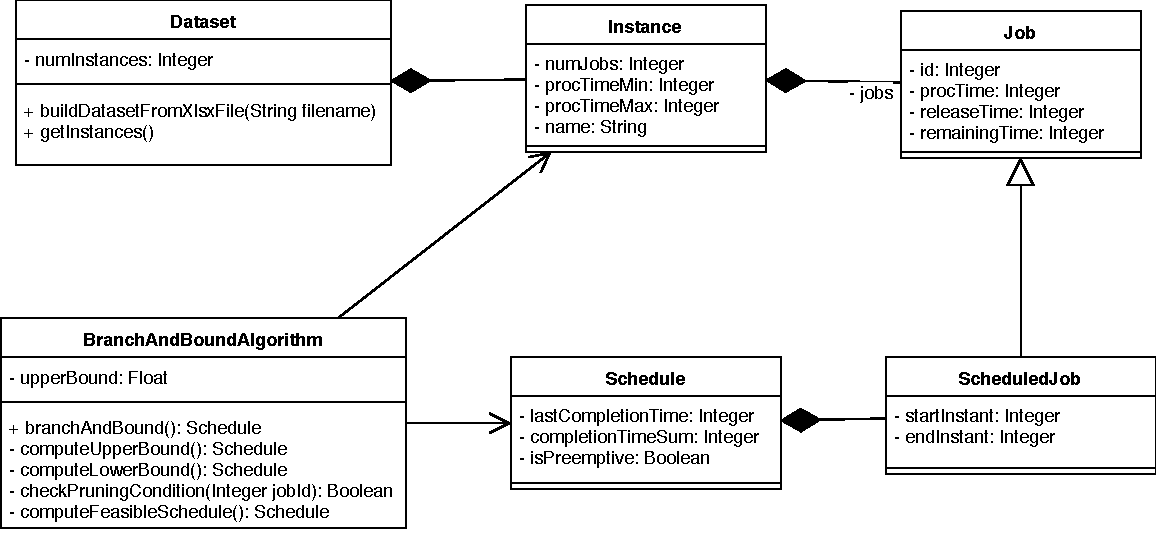
\includegraphics[scale=0.6]{schema_classi.pdf}

\section{Risultati sperimentali}
Presentiamo ora i risultati dei test svolti sulle varie istanze, considerando prima le soluzioni dell'implementazione in Java e poi in AMPL.
\subsection{Schema implementato in Java}
\begin{itemize}
	\item Istanza 1: $\sum_{j} C_j = 3520$%, schedula ottima $\sigma = (8, 2, 6, 7, 5, 1, 10, 3, 9, 4)$
	\item Istanza 2: $\sum_{j} C_j = 15177$%, schedula ottima $\sigma = (29, 9, 14, 16, 25, 7, 12, 17, 8, 28, 19, 27, 3, 11, 26, 30, 24, 20, 2, 15, 21, 4, 10, 6, 18, 5, 23, 13, 1, 22)$
	\item Istanza 3: $\sum_{j} C_j = 9694$%, schedula ottima $\sigma = (7, 19, 23, 16, 4, 12, 28, 21, 9, 26, 11, 3, 5, 17, 30, 6, 8, 10, 24, 2, 22, 13, 15, 27, 29, 18, 14, 25, 20, 1)$
	\item Istanza 4: $\sum_{j} C_j = 32688$%, schedula ottima $\sigma = (35, 14, 1, 33, 8, 38, 40, 6, 30, 23, 11, 32, 13, 21, 12, 17, 2, 28, 34, 29, 16, 18, 15, 10, 24, 5, 20, 3, 39, 22, 36, 37, 31, 27, 19, 25, 4, 7, 26, 9)$
	\item Istanza 5: $\sum_{j} C_j = 16236$%, schedula ottima $\sigma = (3, 30, 11, 25, 38, 13, 31, 26, 39, 14, 4, 20, 12, 24, 27, 37, 23, 6, 29, 9, 32, 33, 15, 1, 10, 8, 5, 21, 16, 22, 19, 18, 36, 40, 2, 17, 28, 34, 7, 35)$
	\item Istanza 6: $\sum_{j} C_j = 87651$%, schedula ottima $\sigma = (40, 8, 36, 30, 3, 51, 33, 43, 20, 52, 35, 5, 53, 16, 44, 4, 41, 56, 2, 34, 14, 18, 24, 57, 19, 21, 15, 9, 12, 42, 25, 7, 45, 13, 50, 49, 59, 17, 55, 58, 47, 1, 27, 11, 28, 37, 38, 10, 54, 23, 48, 31, 6, 29, 26, 32, 60, 46, 22, 39)$
\end{itemize}
\subsection{Schema implementato in AMPL}
Test effettuati su un calcolatore dotato di processore Intel Core i3 di terza generazione.
\begin{itemize}
	\item Istanza 1: $\sum_{j} C_j = 3479$
	\item Istanza 2: $\sum_{j} C_j = 16047$
	\item Istanza 3: $\sum_{j} C_j = 9780$
	\item Istanza 4: $\sum_{j} C_j = 34009$
	\item Istanza 5: $\sum_{j} C_j = 16954$
	\item Istanza 6: $\sum_{j} C_j = 87948$
\end{itemize}
\section{Analisi sperimentale}
Dai test si evince che i valori delle soluzioni fornite dalle due implementazioni sono confrontabili. Si ipotizza che lasciando proseguire la computazione per lo schema AMPL sia possibile ottenere soluzioni ottime migliori.
\end{document}